\documentclass{standalone}


\usepackage{tikz}
\usepackage{pgfplots}
\usetikzlibrary{calc}
\pgfplotsset{compat=1.15}
\usetikzlibrary{shapes,arrows.meta}
\begin{document}


% The block diagram code is probably more verbose than necessary
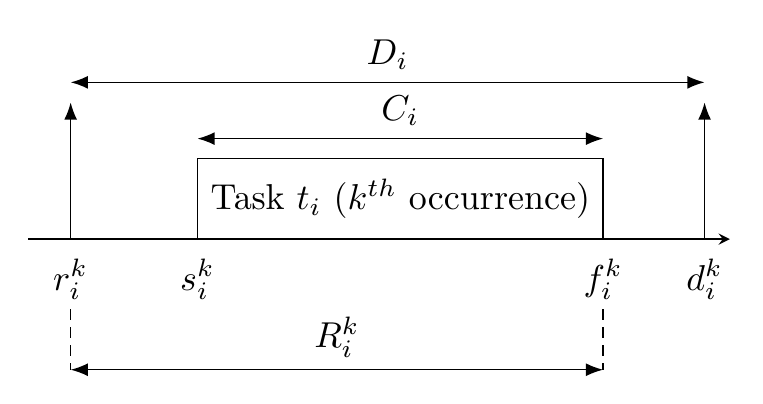
\begin{tikzpicture}[scale=1.3,>=Latex]


\begin{axis}[
    xmin=0, xmax=4.15,
    axis x line=bottom,% only show the bottom x axis
    hide y axis,
		axis lines=middle,
    ymax=2,ymin=-.9,
				xticklabels={$r_{i}^k$,$s_{i}^k$,$f_{i}^k$,$d_{i}^k$},
				xtick={0.25,1,3.4,4},
				%x post scale=1.8
				xtick style={draw=none}
    ]
		
		
\addplot+[mark=none,const plot,draw=black]
coordinates
{(0.25,0) (1,0) (1,0.4) (3.4,0.4) (3.4,0) (4,0)};
\node at(2.2,0.2) {Task $t_i$ ($k^{th}$ occurrence)};
 
\draw [<->] (1,.5) -- node[above] {$C_i$} (3.4,.5);
\draw [<->] (.25,.78) -- node[above] {$D_i$} (4,.78);
\draw [->] (.25,0) -- (.25,.68);
\draw [->] (4,0) -- (4,.68);
\draw [densely dashed](.25,-.35) -- (.25,-.65); 
\draw [densely dashed](3.4,-.35) -- (3.4,-.65);
\draw [<->] (.25,-.65) -- node[above] {$R_{i}^k$} (3.4,-.65); 

\end{axis}
 
\end{tikzpicture}

\end{document}